\section{\multidogo Dataset Curation}

\textit{Generating} and \textit{annotating} a dataset of this scale requires extensive design prior to the task, collection, and post-task quality control.  

\begin{figure*}
	\centering
	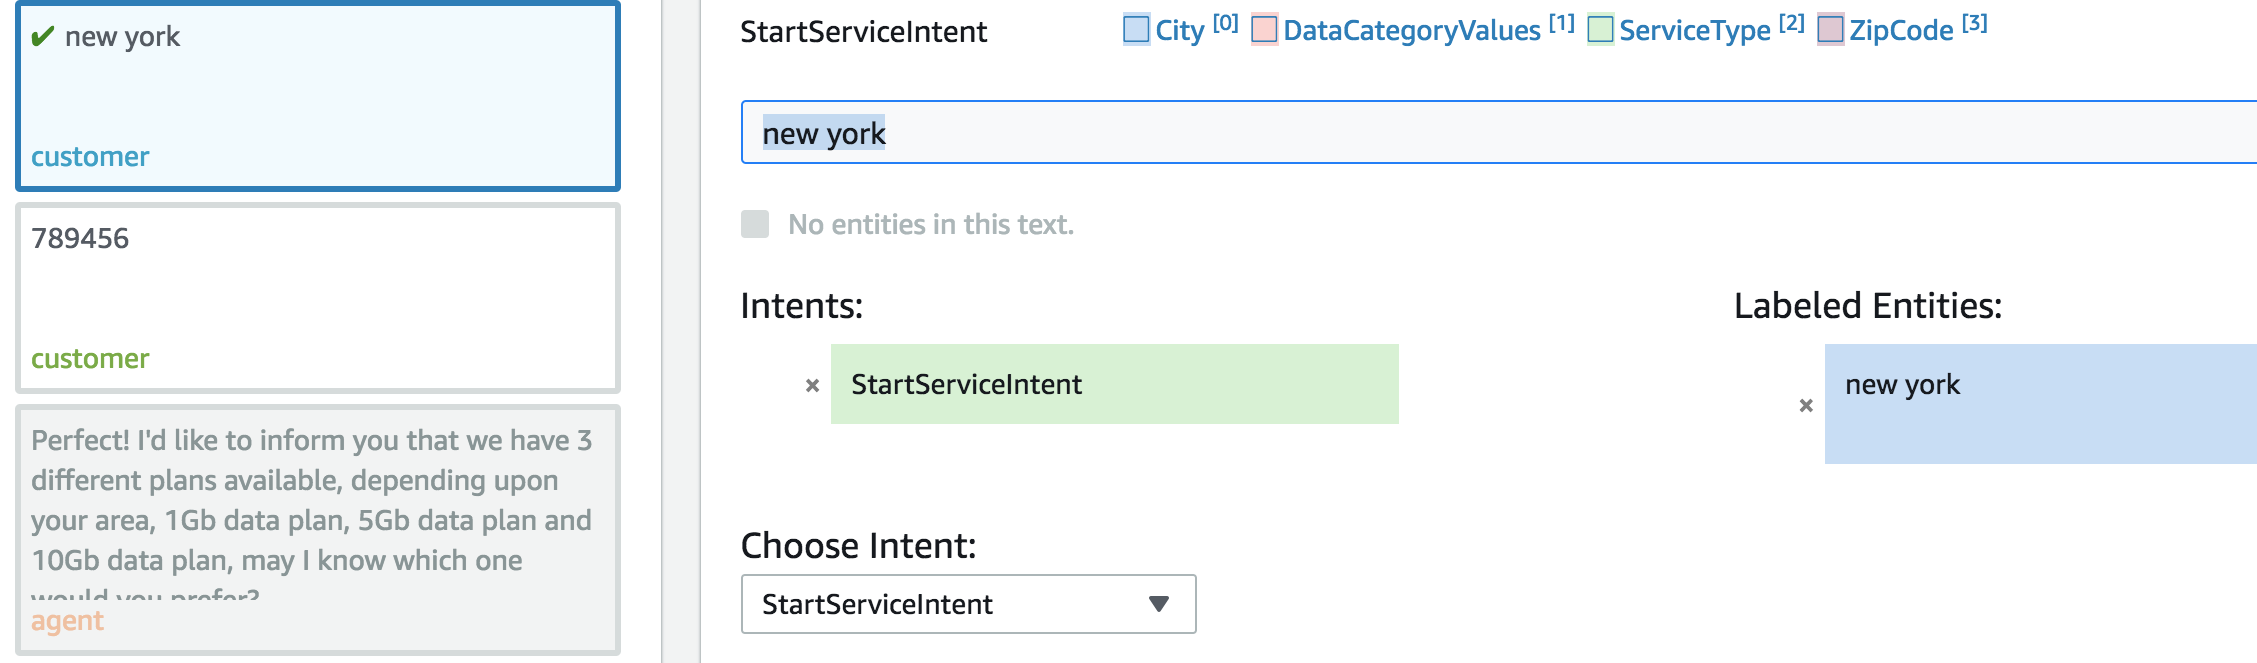
\includegraphics[width=\linewidth]{denis_proposal/sections/multidogo/figures/ic_sl-v3.png}
	\caption{Crowd sourced annotators select an intent and choose a slot in our custom-built Mechanical Turk interface.  Entire conversations are provided for reference.  Detailed instructions are provided to users, but are not included in this figure. Options are unique per domain.}%  There is a separate interface for data generation.}%%Nancy what is the data generation being referenced here?
	\label{fig:SlotAnnotation}
\end{figure*}
%\section{Design Decisions}\label{sec:motivation}

\subsection{Data Collection Procedure}
We employ both internal data associates, who we train,  and crowd-sourced workers from Mechanical  Turk  (MTurkers)  to  generate  conversational data using a Wizard-of-Oz approach. In each conversation, the data associates assumes the role of an agent while the MTurkers act as customers.  In an  effort  to  source  competent  MTurkers,  we  re-quire  that  each  MTurker  have  a  Human  Intelligence  Task  (HIT)  accuracy  minimum  of  90\%,  a location in the United States, and have completed a significant number of HITs in the past. To facilitate goal-oriented conversations between the customer  and  agent,  we  give  each  agent  a  prompt listing  the  supported  request  types  (dialog  acts)and pieces of information (slots) needed to complete each request.  We also specify criteria such as minimal conversation length, number of goals,number of complex requests, etc, to increase conversation diversity.  See Figure 2 for an example prompt. In addition, we explicitly request that neither agents nor customers use any personally identifiable information.  At an implementation level,we create a custom, web interface for the MTurkers and data associates that displays our instructions next to the current dialogue. This allows each participant to quickly refer to our guidelines with-out stopping the conversation.
Despite following a familiar wizard-of-oz elicitation procedure, and curating data for multiple domains in a fashion similar to previous data collection efforts such as \multiwoz, \multidogo comprises more varied domains, it is collected at an unprecedented scale, and it is curated with control over generating explicit biases in the conversations to allow for diverse conversation representation. To our knowledge this is a novel collection strategy as we explicitly guide/prod the participants in a dialogue to engage in conversations with specific biases such as intent change, slot change, multi-intent, multiple slot values, slot overfilling and slot deletion. 
For example, in the Fast Food domain, participants were instructed to pretend that they were ordering fast food from a drive-thru. After making their initial order, they were instructed to change their mind about what they were ordering:``I'd like a burger. No wait, can you make that a chicken sandwich?''. In the Financial domain, we asked participants to make sure that they requested multiple intents such as ``I'd like to find my routing number and check my balance.''\footnote{For a full list of conversational biases with examples, please see the appendix.}
%%NANCY lets add here a paragraph listing all the biases with a couple of examples and then a reference to the appendix for the exhaustive list
To that end, our collection procedure deliberately attempts to guide the dialogue flow to ensure diversity in dialogue policies.


